\section{Results and Discussion}
System-level simulation was performed with representative AI inference workloads.

\subsection{Standby Power}
Migrating cold data and checkpoints to the FeRAM-backed tier yields more than 30\% reduction in standby power.
This reduction arises from suppressing periodic DRAM refresh for inactive regions.

\subsection{Resume Latency}
FeRAM allows direct restore of checkpoints without full DRAM wake-up.
Resume latency is reduced to the $\mu$s range, enabling near-instant resume after power gating and improving energy efficiency for mobile edge AI.

\subsection{Endurance}
FeRAM endurance of $10^{12}$~writes/year fits within FeRAM capability for checkpoint traffic.

% ===== Fig.2: Access time vs. Retention =====
\begin{figure}[!t]
\centering
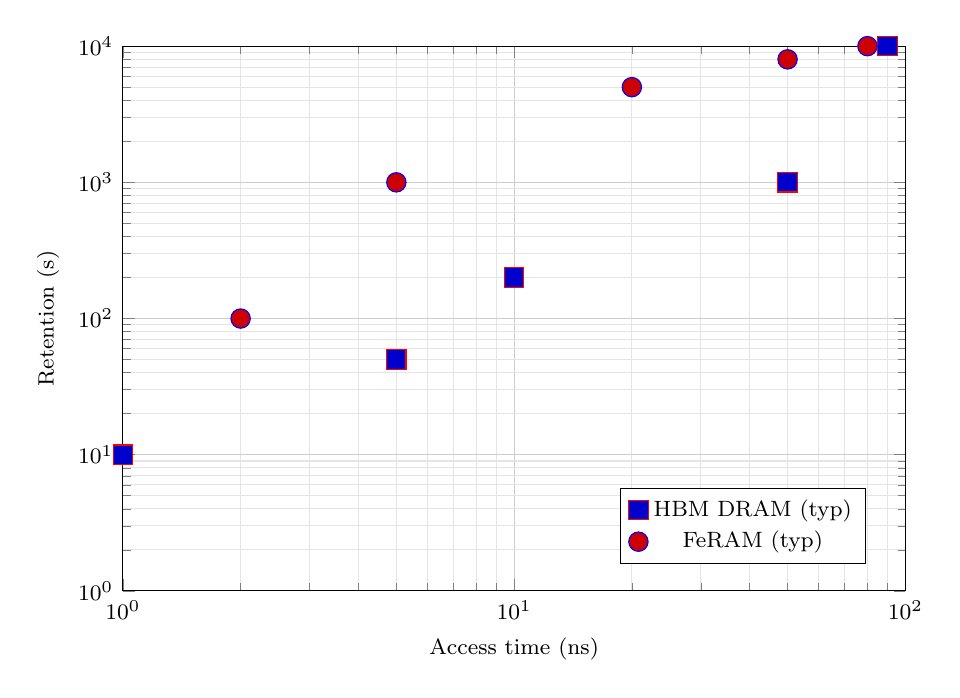
\begin{tikzpicture}
\begin{axis}[
    width=0.95\linewidth,
    height=8.5cm,
    xlabel={Access time (ns)},
    ylabel={Retention (s)},
    xmode=log, ymode=log,
    xmin=1e0, xmax=1e2,
    ymin=1e0, ymax=1e4,
    grid=both,
    major grid style={gray!40},
    minor grid style={gray!20},
    legend style={
        at={(0.95,0.05)},
        anchor=south east,
        font=\footnotesize,
        fill=white,
        draw=black
    },
    tick label style={font=\footnotesize},
    label style={font=\footnotesize}
]

% --- HBM: 赤四角 (塗りつぶしも赤) ---
\addplot+[only marks, mark=square*, mark size=3.5pt, red, fill=red]
coordinates {(1, 10) (5, 50) (10, 200) (50, 1000) (90, 10000)};

% --- FeRAM: 青丸 (塗りつぶしも青) ---
\addplot+[only marks, mark=*, mark size=3.5pt, blue, fill=blue]
coordinates {(2, 100) (5, 1000) (20, 5000) (50, 8000) (80, 10000)};

\legend{HBM DRAM (typ), FeRAM (typ)}
\end{axis}
\end{tikzpicture}
\caption{Access time vs. retention. HBM: red filled squares; FeRAM: blue filled circles. Wider and taller view for clarity ($10^0$--$10^2$ ns, $10^0$--$10^4$ s).}
\label{fig:retention}
\end{figure}
